\scanpage{154}
{\ttfamily\unsure{//CRAY2} JOB '*********',\\
// MSGLEVEL=(1,1),MSGCLASS=A\\
// EXEC PGM=IEFBR14\qquad JOB 0025}
\figure{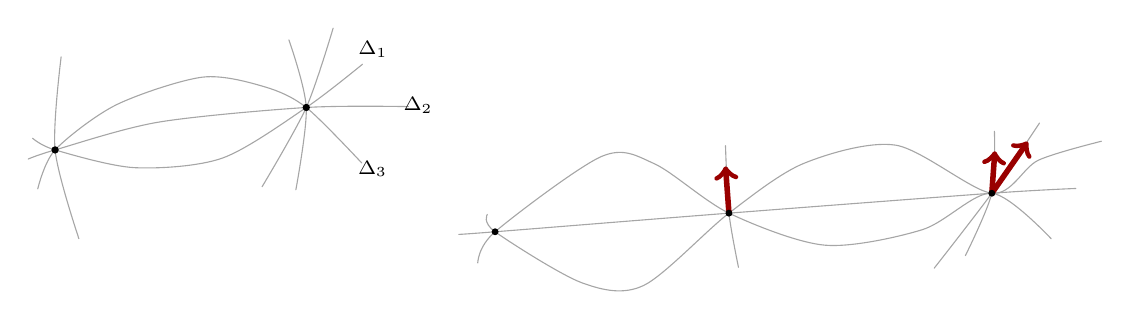
\begin{tikzpicture}[x=.55cm,y=-.55cm,line cap=round,line join=round,g/.style={olive!80!yellow,line width=1.7pt},r/.style={orange!80!brown,line width=1.8pt},w/.style={red!60!black,line width=1.5pt},b/.style={blue!60!black,line width=1.4pt},p/.style={gray!70,thin},k/.style={black,line width=1.2pt},every node/.style={font=\scriptsize}]
\draw[p] plot[smooth] coordinates {(2.7,3.96) (3.32,3.75) (5.7,3.11) (9.12,2.77) (11.48,2.75)};
\draw[p] plot[smooth] coordinates {(2.92,4.65) (3.32,3.75) (4.73,2.71) (6.72,2.07) (8.15,2.29) (9.12,2.77) (10.4,4.05)};
\draw[p] plot[smooth] coordinates {(2.8,3.48) (3.32,3.75) (5.16,4.16) (7.18,3.94) (9.12,2.77) (10.42,1.77)};
\draw[p] plot[smooth] coordinates {(3.46,1.6) (3.32,3.75) (3.87,5.8)};
\draw[p] plot[smooth] coordinates {(8.72,1.21) (9.12,2.77) (8.88,4.67)};
\draw[p] plot[smooth] coordinates {(9.74,.94) (9.12,2.77) (8.1,4.6)};
\fill[k] (3.32,3.75) circle (.085);
\fill[k] (9.12,2.77) circle (.085);
\node at (10.66,1.43) {$\Delta_1$};
\node at (11.7,2.72) {$\Delta_2$};
\node at (10.65,4.19) {$\Delta_3$};
\draw[p] plot[smooth] coordinates {(12.64,5.7) (13.48,5.64) (18.88,5.21) (24.95,4.75) (26.89,4.64)};
\draw[p] plot[smooth] coordinates {(13.08,6.36) (13.48,5.64) (15.94,3.9) (17.16,4.07) (18.88,5.21) (21.1,5.95) (23.35,5.59) (24.95,4.75) (26.32,5.8)};
\draw[p] plot[smooth] coordinates {(13.3,5.24) (13.48,5.64) (15.49,6.82) (16.91,6.88) (18.88,5.21) (20.61,4.06) (22.73,3.64) (24.95,4.75) (26.02,3.99) (27.48,3.55)};
\draw[p] plot[smooth] coordinates {(18.8,3.65) (18.88,5.21) (19.1,6.46)};
\draw[p] plot[smooth] coordinates {(25.01,3.32) (24.95,4.75) (24.34,6.19)};
\draw[p] plot[smooth] coordinates {(26.05,3.13) (24.95,4.75) (23.62,6.48)};
\draw[w,->,line width=2pt] plot[smooth] coordinates {(18.88,5.21) (18.8,4.13)};
\draw[w,->,line width=2pt] plot[smooth] coordinates {(24.95,4.75) (25.02,3.78)};
\draw[w,->,line width=2pt] plot[smooth] coordinates {(24.95,4.75) (25.78,3.56)};
\fill[k] (13.48,5.64) circle (.08);
\fill[k] (18.88,5.21) circle (.08);
\fill[k] (24.95,4.75) circle (.08);
\end{tikzpicture}}

Soit $D$ position relative non principale,
$S_D$ \inserted{$=D\cap S$} \unsure{l'ens.} des sommets multiples de $D$ $(\operatorname{card}S_D\geq2)$.

1) Toute position relative \uline{principale} \inserted{(donc critique)} qui passe par $S_D$ est-elle une spécialisation de $D$ ?

Pour celles \inserted{$\unsure{D'}=\unsure{D'_\delta}$} qui sont des spécialisations de $D$ (\uline{NB} elles ne sont \uline{pas} supracritiques), à chacune d'elle est associé un système de flèches d'orientation des $\Delta_s$ $(s\in S_{\unsure{D'}}\setminus S_D)$ qui ``\unsure{pointent}'' vers $\delta$, et un sens pour parcourir les $\Delta_\sigma$ $(\sigma\in S_D)$.
Pour un $\delta$ donné, ce système de flèches détermine \unsure{déjà} $D$.
\[
\prod_{s\in S_{D'}\setminus S_D}\varepsilon_{\deleted{\unsure{\delta}}D',s}
\qquad \deleted{\unsure{s}}
\]
Il y a aussi le système des \deleted{\unsure{flèches}} \inserted{p.r. stbles} qui générisent $D$,

Les générisations stbles de $D$ correspondent aux sommets d'un cube \unsure{canon.} de dim $\nu$, dont les \unsure{arêtes} sont les générisations semi-stbles, et la relation d'incidence entre sommets et arêtes est la relation de spécialisation.
\figure{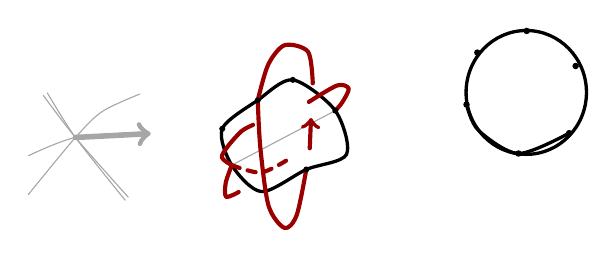
\begin{tikzpicture}[x=.55cm,y=-.55cm,line cap=round,line join=round,g/.style={olive!80!yellow,line width=1.7pt},r/.style={orange!80!brown,line width=1.8pt},w/.style={red!60!black,line width=1.5pt},b/.style={blue!60!black,line width=1.4pt},p/.style={gray!70,thin},k/.style={black,line width=1.2pt},every node/.style={font=\scriptsize}]
\draw[p] plot[smooth] coordinates {(8.86,19.4) (9.94,18.98) (11.5,18.86)};
\draw[p] plot[smooth] coordinates {(8.85,20.3) (9.94,18.98) (10.56,18.38) (11.42,17.98)};
\draw[p] plot[smooth] coordinates {(9.29,17.95) (9.94,18.98) (11.09,20.43)};
\draw[p] plot[smooth] coordinates {(9.2,18.01) (9.94,18.98) (11.16,20.36)};
\draw[p,->,line width=2pt] plot[smooth] coordinates {(9.94,18.98) (11.68,18.89)};
\draw[k] plot[smooth cycle] coordinates {(13.33,18.78) (14.15,18.12) (14.96,17.65) (15.94,18.36) (16.2,19.37) (15.27,19.72) (14.24,20.23) (13.55,19.62)};
\draw[p] plot[smooth] coordinates {(13.55,19.62) (15.94,18.36)};
\draw[w] plot[smooth] coordinates {(14.15,18.12) (14.39,17.3) (14.77,16.85) (15.31,17.0) (15.42,17.73)};
\draw[w] plot[smooth] coordinates {(15.33,18.16) (15.98,17.78) (16.25,17.85) (16.1,18.17) (15.94,18.36)};
\draw[w] plot[smooth] coordinates {(14.15,18.12) (14.21,19.22) (14.4,20.56) (14.77,21.07) (15.05,20.77) (15.27,19.72)};
\draw[w] plot[smooth] coordinates {(13.55,19.62) (13.32,19.44) (13.47,19.17) (13.78,18.83) (14.04,18.69)};
\draw[w] plot[smooth] coordinates {(13.55,19.62) (13.41,20.03) (13.42,20.35) (13.71,20.24)};
\draw[w,dashed] plot[smooth] coordinates {(13.55,19.62) (14.22,19.79) (14.83,19.5)};
\draw[w,->] plot[smooth] coordinates {(15.35,19.23) (15.38,18.53)};
\fill[k] (13.33,18.78) circle (.07);
\fill[k] (14.15,18.12) circle (.07);
\fill[k] (14.96,17.65) circle (.07);
\fill[k] (15.94,18.36) circle (.07);
\fill[k] (15.27,19.72) circle (.07);
\draw[k] (20.35,17.94) ellipse (1.39 and 1.43);
\draw[k] plot[smooth] coordinates {(18.97,18.22) (19.24,18.81) (20.17,19.35) (21.34,18.88)};
\fill[k] (19.22,17.02) circle (.075);
\fill[k] (20.36,16.52) circle (.075);
\fill[k] (21.49,17.33) circle (.075);
\fill[k] (21.34,18.88) circle (.075);
\fill[k] (20.17,19.35) circle (.075);
\fill[k] (18.97,18.22) circle (.075);
\end{tikzpicture}}

\unsure{Produit} des diagonales d'un polygone \inserted{\unsure{convexe}} \unsure{régulier}
\deleted{degré} $2\nu$.
\[
2^{\nu\unsure{+}}\ \text{sommets},\quad \nu2^{\nu-1}\ \text{arêtes}
\]
\margin{\mspage{153}}
